\documentclass[MGS,Seminar,ngerman]{twbook}%\documentclass[Bachelor,BMR,ngerman]{twbook}
\usepackage[utf8]{inputenc}
\usepackage[T1]{fontenc}
\usepackage{float}

%
% Bitte in der folgenden Zeile den Zitierstandard festlegen
\newcommand{\FHTWCitationType}{IEEE} % IEEE oder HARVARD möglich - wenn Sie zwischen IEEE und HARVARD wechseln, bitte die temorären Dateien (aux, bbl, ...) löschen
%
\ifthenelse{\equal{\FHTWCitationType}{HARVARD}}{\usepackage{harvard}}{\usepackage{bibgerm}}

% Definition Code-Listings Formatierung:
\usepackage[final]{listings}
\lstset{captionpos=b, numberbychapter=false,caption=\lstname,frame=single, numbers=left, stepnumber=1, numbersep=2pt, xleftmargin=15pt, framexleftmargin=15pt, numberstyle=\tiny, tabsize=3, columns=fixed, basicstyle={\fontfamily{pcr}\selectfont\footnotesize}, keywordstyle=\bfseries, commentstyle={\color[gray]{0.33}\itshape}, stringstyle=\color[gray]{0.25}, breaklines, breakatwhitespace, breakautoindent}
\lstloadlanguages{[ANSI]C, C++, [gnu]make, gnuplot, Matlab}

%Formatieren des Quellcodeverzeichnisses
\makeatletter
% Setzen der Bezeichnungen für das Quellcodeverzeichnis/Abkürzungsverzeichnis in Abhängigkeit von der eingestellten Sprache
\providecommand\listacroname{}
\@ifclasswith{twbook}{english}
{%
    \renewcommand\lstlistingname{Code}
    \renewcommand\lstlistlistingname{List of Code}
    \renewcommand\listacroname{List of Abbreviations}
}{%
    \renewcommand\lstlistingname{Quellcode}
    \renewcommand\lstlistlistingname{Quellcodeverzeichnis}
    \renewcommand\listacroname{Abkürzungsverzeichnis}
}
% Wenn die Option listof=entryprefix gewählt wurde, Definition des Entyprefixes für das Quellcodeverzeichnis. Definition des Macros listoflolentryname analog zu listoflofentryname und listoflotentryname der KOMA-Klasse
\@ifclasswith{scrbook}{listof=entryprefix}
{%
    \newcommand\listoflolentryname\lstlistingname
}{%
}
\makeatother
\newcommand{\listofcode}{\phantomsection\lstlistoflistings}

% Die nachfolgenden Pakete stellen sonst nicht benötigte Features zur Verfügung
\usepackage{blindtext}
%
% Einträge für Deckblatt, Kurzfassung, etc.
%
\title{Algorithmen zur Fragmentierung von 3D-Objekten}
\author{Michael Prommer, BSc}
\studentnumber{1910585010}
%\author{Titel Vorname Name, Titel\and{}Titel Vorname Name, Titel}
%\studentnumber{XXXXXXXXXXXXXXX\and{}XXXXXXXXXXXXXXX}
\supervisor{Titel Vorname Name, Titel}
%\supervisor[Begutachter]{Titel Vorname Name, Titel}
%\supervisor[Begutachterin]{Titel Vorname Name, Titel}
%\secondsupervisor{Titel Vorname Name, Titel}
%\secondsupervisor[Begutachter]{Titel Vorname Name, Titel}
%\secondsupervisor[Begutachterinnen]{Titel Vorname Name, Titel}
\place{Wien}
\kurzfassung{\blindtext}
\schlagworte{Schlagwort1, Schlagwort2, Schlagwort3, Schlagwort4}
% \outline{\blindtext}
% \keywords{Keyword1, Keyword2, Keyword3, Keyword4}
%\acknowledgements{\blindtext}

\begin{document}

%Festlegungen für den HARVARD-Zitierstandard
\ifthenelse{\equal{\FHTWCitationType}{HARVARD}}{
\bibliographystyle{Harvard_FHTW_MR.bst}%Zitierstandard FH Technikum Wien, Studiengang Game Engineering
\citationstyle{dcu}%Correct citation-style (Harvardand, ";" between citations, "," between author and year)
\citationmode{abbr}%use "et al." with first citation
\iflanguage{ngerman}{
    %Deutsch Neue Rechtschreibung
    \newcommand{\citepic}[1]{(Quelle: \protect\cite{#1})}%Zitat: Bild
    \newcommand{\citefig}[2]{(Quelle: \protect\cite{#1}, S. #2)}%Zitat: Bild aus Dokument
    \newcommand{\citefigm}[2]{(Quelle: modifiziert "ubernommen aus \protect\cite{#1}, S. #2)}%Zitat: modifiziertes Bild aus Dokument
    \newcommand{\citep}{\citeasnoun}%In-Line Zitiat entweder mit \citep{} oder \citeasnoun{}
    \newcommand{\acessedthrough}{Verf{\"u}gbar unter:}%Für URL-Angabe
    \newcommand{\acessedthroughp}{Verf{\"u}gbar bei:}%Für URL-Angabe (Geschützte Datenbank, Zugriff durch FH)
    \newcommand{\acessedat}{Zugang am}%Für URL-Datum-Angabe
    \newcommand{\singlepage}{S.}%Für Seitenangabe (einzelne Seite)
    \newcommand{\multiplepages}{S.}%Für Seitenangabe (mehrere Seiten)
    \newcommand{\chapternr}{K.}%Für Kapitelangabe
    \renewcommand{\harvardand}{\&}%Harvardand in Zitaten
    \newcommand{\abstractonly}{ausschließlich Abstract}
    \newcommand{\edition}{. Auflage}%Angabe der Auflage
}{
\iflanguage{german}{
    %Deutsch
    \newcommand{\citepic}[1]{(Quelle: \protect\cite{#1})}%Zitat: Bild
    \newcommand{\citefig}[2]{(Quelle: \protect\cite{#1}, S. #2)}%Zitat: Bild aus Dokument
    \newcommand{\citefigm}[2]{(Quelle: modifiziert "ubernommen aus \protect\cite{#1}, S. #2)}%Zitat: modifiziertes Bild aus Dokument
    \newcommand{\citep}{\citeasnoun}%In-Line Zitiat entweder mit \citep{} oder \citeasnoun{}
    \newcommand{\acessedthrough}{Verf{\"u}gbar unter:}%Für URL-Angabe
    \newcommand{\acessedthroughp}{Verf{\"u}gbar bei:}%Für URL-Angabe (Geschützte Datenbank, Zugriff durch FH)
    \newcommand{\acessedat}{Zugang am}%Für URL-Datum-Angabe
    \newcommand{\singlepage}{S.}%Für Seitenangabe (einzelne Seite)
    \newcommand{\multiplepages}{S.}%Für Seitenangabe (mehrere Seiten)
    \newcommand{\chapternr}{K.}%Für Kapitelangabe
    \renewcommand{\harvardand}{\&}%Harvardand in Zitaten
    \newcommand{\abstractonly}{ausschließlich Abstract}
    \newcommand{\edition}{. Auflage}%Angabe der Auflage
}{
    %Englisch
    \newcommand{\citepic}[1]{(Source: \protect\cite{#1})}%Zitat: Bild
    \newcommand{\citefig}[2]{(Source: \protect\cite{#1}, p. #2)}%Zitat: Bild aus Dokument
    \newcommand{\citefigm}[2]{(Source: taken with modification from \protect\cite{#1}, p. #2)}%Zitat: modifiziertes Bild aus Dokument
    \newcommand{\citep}{\citeasnoun}%In-Line Zitiat entweder mit \citep{} oder \citeasnoun{}
    \newcommand{\acessedthrough}{Available at:}%Für URL-Angabe
    \newcommand{\acessedthroughp}{Available through:}%Für URL-Angabe (Geschützte Datenbank, Zugriff durch FH)
    \newcommand{\acessedat}{Accessed}%Für URL-Datum-Angabe
    \newcommand{\singlepage}{p.}%Für Seitenangabe (einzelne Seite)
    \newcommand{\multiplepages}{pp.}%Für Seitenangabe (mehrere Seiten)
    \newcommand{\chapternr}{Ch.}%Für Kapitelangabe
    \renewcommand{\harvardand}{\&}%Harvardand in Zitaten
    \newcommand{\abstractonly}{Abstract only}
    \newcommand{\edition}{~edition}%Edition -> note, that you have to write "edition = {2nd},"!
}}}

\maketitle
%
% .. und hier beginnt die eigentliche Arbeit. Viel Erfolg beim Verfassen!
%

\chapter{Einführung}

In modernen Videospielen und Filmen werden verschiedenste Effekte verwendet um dem Spieler die Welt glaubhafter und realer wirken zu lassen.
Einer davon ist die Zerstörung von unterschiedlichen Objekten im Spiel wie einfache Gegenstände oder in manchen Spielen sogar zerstörbare Landschaften.
Aufgrund des hohen Rechenaufwands wird in Spielen jedoch meist ein statischer und nicht physikalischer Ansatz für solch destruktive Objekte verwendet, 
das heißt ein Model wird von einem Artist bereits vorher fragmentiert modelliert und zum gewünschten Zeitpunkt im Spiel einfach ausgetauscht. 
Dieser Ansatz hat jedoch auch Nachteile. Zum Beispiel wird die Entwicklungszeit eines Spieles verlängert, da der Artist 3D-Modelle mit 
unterschiedlichen Frakturierungen erstellen muss, und zusätzlich kann es sein, dass die Spielerinteraktion in der Spielumgebung durch 
vorgebrochene Objekte einteschränkt wird \cite{Najim.DynamicFracturing}.
Außerdem hat diese Methode den Nachteil, dass das Muster der Fragmentierung nicht mit der Einschlagstelle übereinstimmt und dass die Anzahl der 
hierarchischen Burchstufen bereits festgelegt ist \cite{Mueller.RealTimeDynamicFractureVACD}. Um eine physikalisch korrekte Fragmentierung zu erhalten, muss man 
auch auf physikalisch basierte Methoden zurückgreifen. Mithilfe dieser Methoden ist es zwar möglich realistische Simulationen durchzuführen, doch aufgrund des hohen
Rechenaufwandes sind diese Methoden meist nicht für interraktive Programme, wie beispielsweise Videospiele, anwendbar \cite{Torres.FractureModelingSurvey}.
Aber aufgrund von intensiver Forschung von physikalischen Methoden, ist es mittlerweile sogar möglich einige dieser Methoden in Echtzeit auszuführen wie beispielsweise
Parker und O'Brien \cite{Parker.Real-TimeDeformation} zeigen.

Durch bisherige Bemühungen auf diesem Gebiet konnten nicht physikalisch basierte Algorithmen entwickelt werden, welche in Echtzeit ausgeführt werden, ein 
realischtisches Ergebnis erzielen und dadurch einen dynamischeren Effekt erzielen. 
Deshalb können beispielsweise interessantere und nicht repetitive Fragmentierungsmuster erstellt werden und außerdem fällt die 
Entwicklungszeit der 3D-Modellen mit unterschiedlichen Frakturierungen weg.
Diese Algorithmen zur Erstellung von Fragmentierungen basieren meist auf dem sogenannten Voronoi Diagramm.\\

\chapter{State of the Art}

In diesem Abschnitt werden aktuelle Methoden erläutert um ein 3D-Objekt zu fragmentieren. Dabei wird unterschieden zwischen nicht physikalisch basierten und
physikalisch basierten Methoden. 

\section{Nicht Physikalisch basierte Methoden}

Nicht physikalisch basierte Methoden versuchen, realistische Burchmuster zu reproduzieren, ohne den grundlgegenden physikalischen Prozess zu berücksichtigen.
Ein Beispiel davon wären Bildbasierte Methoden, welche ein Eingabebild oder eine Textur nutzen, um reale Bruchmuster zu erfassen 
und zu übertragen \cite{Torres.FractureModelingSurvey}.

Mould \cite{Mould.Image-guidedFracture} entwickelte einen Algorithmus, welcher eine Zeichung einer Linie als Input nimmt und in ein Bild 
einer gebrochenen Oberfläche transformiert, wobei die Risse die Zeichnung reproduzieren, wie in folgender Abbildung \ref{fig:imagebasedVoronoi} zu erkennen ist.

\begin{figure}[H]
    \centering
    
\includegraphics[width=0.45\linewidth]{PICs/imagebasedFractureVoronoi.PNG}
    \caption{Ein Text als Eingabe für den Algorithmus und darunter das resultierene Bruchmuster, wobei der Text noch zu erkennen ist
    \protect\cite{Mould.Image-guidedFracture}}.
    \label{fig:imagebasedVoronoi}
\end{figure}

%Wie schon bereits erwähnt wird in den nicht physikalisch basierten Methoden meist auf das Voronoi Diagramm zurückgegriffen. 
Dadurch, dass in diesem Algorithmus und in vielen anderen Fragmentierungsmethoden das Voronoi Diagramm zum Einsatz kommt, folgt eine Defintion und Beschreibung 
des Voronoi Diagrams.

Ausgehend von einer endlichen Menge an verschiedenen, isolierten Punkten in einem Raum, werden alle Orte mit dem nächstgelegenen Punkt der Punktmenge assoziiert.
Das Ergebnis ist eine Unterteilung des Raumes in eine Menge von Regionen, die sogenannten Voronoi Zellen, die zusammen das Voronoi Diagramm bilden, 
wie in Abbildung \ref{fig:voronoi1} zu sehen ist \cite{Okabe.SpatialTessellationsVoronoi}.


\begin{figure}[H]
    \centering
    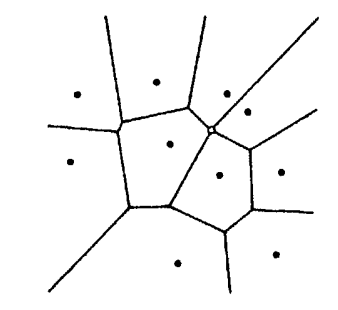
\includegraphics[width=0.35\linewidth]{PICs/basicVoronoi.PNG}
    \caption{Voronoi Diagramm \protect\cite{Okabe.SpatialTessellationsVoronoi}}
    \label{fig:voronoi1}
\end{figure}

Diese Voronoi Zellen werden als Primitive genutzt, um zerstörbare 3D Regionen zu repräsentieren, können schnell und einfach berechnet werden und auf praktisch alle 3D-Modelle
angewendet werden \cite{Najim.DynamicFracturing}.

Um nun Risse, Brüche oder Fragmente zu erzeugen wird ein Voronoi Diagramm konstruiert, indem im Innenraum und an den Kanten jedes Polygons zusätzliche Punkte erzeugt werden. 
Anschließend wird die resultierende Punktemenge trianguliert, inklusive der Kanten des Polygons, und infolgedessen das Voronoi Diagramm gebildet. 
Zum Schluss werden jene Kanten des Voronoi Netzes ausgeschnitten, welche über das Polygon hinausgehen. Das Ergebnis ist eine Sammlung von kleineren Polygonen, die zusammen
das ursprüngliche Polygon ergeben \cite{Raghavachary.FractureGenerationOnPolygonalMeshes}.

\begin{figure}[H]
    \centering
    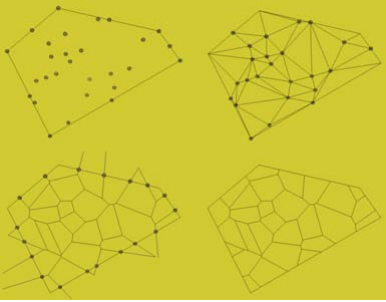
\includegraphics[width=0.5\linewidth]{PICs/voronoiSteps.PNG}
    \caption{Erstellung eines Voronoi Netzwerkes bei einem Polygon \protect\cite{Raghavachary.FractureGenerationOnPolygonalMeshes}}
    \label{fig:voronoi2}
\end{figure}

In Abbildung \ref{fig:voronoi2} werden die oben genannten Schritte grafisch dargestellt.

Um nun Verfeinerungen bei der Fragmentierung des Polygons an bestimmten Stellen vorzunehmen, muss nur die Punktmenge an eben diesen Stellen erhöht werden. Dadurch ergeben
sich bei der Erstellung des Voronoi Diagramms kleinere Polygone. Dies ist nützlich um beispielsweise den Eintreffpunkt eines Projektiles, oder 
den Auftreffpunkt eines herunterfalllenden Gegenstandes genau zu definieren. 




% genralized in a variety of ways (chapter 3 in okabe)
% data structures to represent voronoi (chapter 4)


\section{Physikalisch basierte Methoden}

%physikalische Methoden 
Aufgrund der realistischen Fragmentierung und hohen Berechnungszeit der physikalischen Methoden, werden diese häufig bei Simulationen eingesetzt,
um akkurate Resultate zu erzielen. Mittlerweile wurden jedoch neue Methoden entwickelt beziehungsweise die bestehenden Methoden erweitert und perfektioniert 
und finden sich auch in Videospielen wieder. 

\subsection{Mass-Spring Model}

Grundlegend basiert die Technik des Mass-Spring Models darauf, dass bestimmte Punkte eines 3D-Objektes mit Sprungfedern miteinander verbunden sind und entfernt werden, 
sobald diese einer bestimmten Belastung ausgesetzt sind. 
Diese Belastung basiert auf einer bestimmten Schwelle die abhängig ist von der Länge der Feder und des Materials des 3D-Objektes. Ein Nachteil dieser Methode ist,
dass die Position und Rotation der Bruchstelle unbekannt ist.

Mazarak et al \cite{Mazarak.AnimatingExplodingObjects} haben diesen Algorithmus erweitert, indem sie einen Voxel basierten Ansatz verwendet haben,
um solide Objekte zu modellieren. Das bedeutet das Voxel miteinander verbunden sind, und diese Verbindungen starr sind, um benachbarte 
Voxel stark miteinander verbunden zu halten. 
Diese verbundenen Voxel können nun zu gemeinsamen Körpern verbunden werden. Anschließend können diese Körper gruppiert werden, um bestimmte Formen oder Objekte zu bilden.
Eine Fragmentierung wird nun simuliert, indem Verbindungen zwischen den Körpern gebrochen werden.

\subsection{Finite-Element Methode}

Im Gegensatz zum Mass-Spring Model, welches von diskreter Natur ist, wird die Finite-Element-Methode(FEM) aus den Gleichungen der Kontinuumsmechanik abgeleitet.
Hauptsächlich wird dabei das Objekt in kleine, miteinander verbundene Bereiche, die sogenannten finiten Elemente, unterteilt. 
Innerhalb jedes Elements wird das Objekt mithilfe einer Funktion, mit einer endlichen Anzahl an Paramatern, lokal beschrieben. Diese Funktion wird in eine Menge von
Funktionen mit orthogonaler Form zerlegt, die jeweils einem der Knoten an der Grenze des Elementes zugeordnet sind \cite{OBrien.BrittleFracture}. 

Die Finite-Element Methode wird meist bei Simulationen eingesetzt, jedoch ist es Parker und O'Brien \cite{Parker.Real-TimeDeformation} gelungen
diese Methode in einem Echtzeit Kontext, genauer ausgedrückt in einem kommerziellen Videospiel, anzuwenden.


\chapter{Fazit}

Abschließend

Zusammenfassen

Ausblick(Genauer Performance Unterschied zwischen Methoden)



%
% Hier beginnen die Verzeichnisse.
%
\clearpage
\ifthenelse{\equal{\FHTWCitationType}{HARVARD}}{}{\bibliographystyle{gerabbrv}}
\bibliography{Literatur}
\clearpage

% Das Abbildungsverzeichnis
% \listoffigures
% \clearpage

% Das Tabellenverzeichnis
% \listoftables
% \clearpage

% Das Quellcodeverzeichnis
% \listofcode
% \clearpage

% \phantomsection
% \addcontentsline{toc}{chapter}{\listacroname}
% \chapter*{\listacroname}
% \begin{acronym}[XXXXX]
%     \acro{ABC}[ABC]{Alphabet}
%     \acro{WWW}[WWW]{world wide web}
%     \acro{ROFL}[ROFL]{Rolling on floor laughing}
% \end{acronym}

\end{document}